\documentclass[times, utf8, seminar, numeric]{fer}
\usepackage{booktabs}
\usepackage{multirow}
\usepackage{url}
\usepackage[T1]{fontenc}
\usepackage{caption}
\usepackage{tabularx}
\usepackage{array}
\usepackage{float}
\usepackage{algpseudocode}
\usepackage{algorithm}
\usepackage{pgfplots}

\newcolumntype{P}[1]{>{\centering\arraybackslash}p{#1}}

\renewcommand{\algorithmicforall}{\textbf{for each}}
\pgfplotsset{compat=1.15}
\begin{document}

\nocite{*}

\title{Izgradnja binarnog stabla valića kao RRR strukture}

\author{Jure Čular 0036479001 \and 
        Bartol Freškura 0036480392 \and 
        Filip Gulan 0036479428}

\maketitle{}

\tableofcontents

\chapter{Uvod}
U području bioinformatike mogu se susresti sekvence znakova velikih duljina koje je potrebno obraditi ili izvršavati određene upite nad istima, poput pronalaska broja pojavljivanja određenog znaka do danog indeksa i sličnih. Slijedno obrađivanje navedenih sekvenci bi bilo vrlo sporo i neučinkovito te se poseže za nešto bržim, no i kompliciranijim rješenjima. Jedan od predstavnika je i binarno stablo valića kao RRR struktura koja je obrađena u ovom projektu.

Zadatak ovog projekta je bila izgradnja gore navedene strukture, provedba testiranja nad sintetičkim i stvarnim podacima u vidu brzine izgradnje stabla, potrošnje memorije te prosječnog vremena izvršavanja upita \emph{rank}, \emph{select} i \emph{access}. U nastavku dokumenta je prikazan opis RRR strukture, stabla valića te implementacije istih. Na kraju su dani rezultati i usporedba s onima od prošlogodišnjeg projekta \cite{breberic}.


\chapter{RRR struktura podataka}
RRR je struktura podatka za pohranjivanje bit-vektora pomoću koje je moguće u kratkom vremenu izvršiti upite. Navedena struktura je sažeta \engl{Succint data structure}, no unatoč tomu nije ju potrebno u cijelosti raspakirati kako bi se obavio upit nad istom. 

\section{Izgradnja RRR strukture}

Prilikom izgradnje RRR strukture prvi korak je podjela ulaznog niza bitova na blokove, odnosno superblokove. Veličine superbloka i bloka moguće je proizvoljno definirati. Nakon odabira veličine bloka potrebno je izgraditi RRR tablicu.

\begin{figure}[H]
	\centering
	\includegraphics[width = 0.5\textwidth] {img/rrrtable.png}
	\caption{Sadržaj RRR tablice za $b = 5$, preuzeto iz \cite{breberic}}
	\label{fig:rrrtable}
\end{figure}

Tablica je pomoćna struktura koja će se koristiti u izvršavanju upita. Sama tablica će sadržavati sve moguće permutacije blokova za sve moguće rangove za danu veličinu bloka te niz sume rangova do svake pozicije unutar bloka. Implementacijski gledano tablica će sadržavati pokazivače na tablice za svaki rang bloka unutar kojih će biti definirane permutacije tog ranka i odgovarajuća sumu jedinica za svaku poziciju u odgovarajućem bloku. Primjer jedne takve tablice prikazan je na slici \ref{fig:rrrtable}.

Kroz sljedeći primjer bit će prikazana izgradnja RRR strukture iz ulaznog niza bitova, za veličinu bloka $b=5$ i superbloka $f=2$. Na slici \ref{fig:blocks} je prikazana podjelu niza na četiri bloka i dva superbloka. Nakon podjele niza bitova u blokove i superblokove potrebno je za svaki blok odrediti rang te odmak unutar tablice blokova, odnosno pozicija bloka unutar tablice koji odgovara danom bloku. Tako dobiveni parovi se spremaju u niz koji će se koristiti u daljnjim operacijama nad strukturom. Uz navedeni niz, također se sprema i niz parova koji sadrže ukupnu sumu rangova unutar prethodnih superblokova te odmak prvog bloka za pojedini superblok. 

\begin{figure}[H]
	\centering
	\includegraphics[width=0.6\textwidth]{img/superblocks.pdf}
	\caption{Podjela bit-vektora na blokove i superblokove}
	\label{fig:blocks}
\end{figure} 

Korištenjem tablice \ref{fig:rrrtable} nad primjerom danim na slici \ref{fig:blocks} dobio bi se kodiran niz prikazan u obliku parova $[(3, 4), (1, 4), (2, 2), (1, 2)]$, gdje prvi element para predstavlja rang, a drugi odmak u tablici. Isti taj niz, zapisan kao niz bitova prikazan je na slici \ref{fig:codecseq}. Niz parova suma ranga i odmaka prvog sljedećeg bloka bi ovisio o tome kako se zapisuju navedeni parovi u memoriju. Naime, moguće je navedene parove zapisivati kao dva broja ili ih kodirati tako da se postigne maksimalna memorijska učinkovitost. No takav način kodiranja zahtjeva i dekodiranje prilikom obavljanja upita što može dodatno usporiti brzinu njihova izvršavanja. Razlika u ta dva načina zapisa je u odmaku prvog bloka, za nekodirane nizove odmak je samo indeks prvog slijedećeg bloka, dok za kodirane iznosi broj bitova do odmaka (odmak unutar RRR tablice) prvog slijedećeg bloka. Za primjer dan na slici \ref{fig:blocks} i bez kodiranja taj niz bi iznosio $[(0, 0), (4, 2)]$, dok bi uz kodiranje iznosio $[(0, 3), (4, 16)]$.

\begin{figure}[H]
	\centering
	\includegraphics[width=0.6\textwidth]{img/coded.pdf}
	\caption{Ulazni niz \texttt{10011100000011000100} kodiran u RRR strukturu}
	\label{fig:codecseq}
\end{figure}

\subsection{Kodiranje parova}

Kodiranje parova moguće je izvršiti tako da se uzme broj bitova potrebnih za najveći rang bloka unutar RRR tablice odnosno $r\_bit=\lceil(\log_2(b + 1))\rceil$ gdje je $b$ veličina bitova u bloku, dok se broj bita odmaka uzme veličina koja ovisi o rangu $o\_bit=\lceil(\log_2({b \choose r}))\rceil$ gdje je $r$ rang u bloku. Uz pomoć te dvije veličine moguće je jedan par spremiti unutar $o\_bit+r\_bit$ bitova.

\subsection{Dekodiranje parova}

Dekodiranje parova se vrši na način da se prvo dekodira rang jer je broj bitova za kodiranje ranga stalan te je poznat početak bloka. Nakon dekodiranja ranga, iz RRR tablice možemo saznati potreban broj bitova za odmak te dekodirati i sam odmak.

\section{Upiti nad RRR strukturom}

Nad RRR strukturom moguće je obavljati tri vrste upita:

\begin{itemize}
    \item $rank_b(i) $- broj pojavljivanja bita $b$ do pozicije $i$ u ulaznom nizu bitova
    \item $select_b(i)$ - pozicija $i$-tog pojavljivanja bita $b$ u ulaznom nizu bitova
    \item $access(i)$ - bit na $i$-toj poziciji u ulaznom nizu bitova
\end{itemize}

\subsection{\emph{Rank}}

Nad RRR strukturom možemo obavljati \emph{rank1} i \emph{rank0} upite, gdje \emph{rank1} vraća broj bitova postavljenih na $1$ do danog indeksa u nizu, te \emph{rank0} analogno tomu broj bitova postavljenih na $0$. Algoritam \emph{rank1} i \emph{rank0} upita prikazan je pseudokodom \ref{alg:rrr_rank1} i \ref{alg:rrr_rank0}.

\begin{algorithm}[H]
  \floatname{algorithm}{Pseudokod}
  \caption{\emph{rank1} upit nad RRR strukturom, preuzeto iz \cite{bowe-th} i \cite{breberic}}
  \begin{algorithmic}[1]
    \Function{rank1}{$i$}
    \State $i_b \gets \left \lfloor \frac{i}{b} \right \rfloor$
    \State $i_s \gets \left \lfloor \frac{i_b}{b * s} \right \rfloor$
    \State $suma \gets $ rank $i_s$-tog super bloka
    \State $trenutni\_blok \gets $ prvi blok $i_s$ tog super bloka
    \While{$trenutni\_blok \neq i_b$-ti blok}
      \State $suma \gets suma + $ razred od $trenutni\_blok$
      \State $trenutni\_blok \gets $ slijedeći blok
      \State $j \gets i \ \% \ b$
      \State $suma \gets suma + $ pozicija na kojoj se nalazi $j$-ta jedinica u bloku 
      \State{}
      \Return $suma$
    \EndWhile
    \EndFunction
  \end{algorithmic}
  \label{alg:rrr_rank1}
\end{algorithm}

\begin{algorithm}[H]
  \floatname{algorithm}{Pseudokod}
  \caption{\emph{rank0} upit nad RRR strukturom, preuzeto iz \cite{bowe-th} i \cite{breberic}}
  \begin{algorithmic}[1]
    \Function{rank0}{$i$}
      \State{} \Return $i + 1 - $ \Call{rank1}{$i$}
    \EndFunction
  \end{algorithmic}
  \label{alg:rrr_rank0}
\end{algorithm}


\subsection{\emph{Select}}

Kao i za \emph{rank} upite, nad RRR strukturom možemo izvoditi \emph{select1} i \emph{select0} upite. Oni odgovaraju pozicijom $i$-tog bita postavljenog na $1$, odnosno $0$. Algoritam \emph{select1} i \emph{select0} upita prikazan je pseudokodom \ref{alg:rrr_select1} i \ref{alg:rrr_select0}.

\begin{algorithm}[H]
  \floatname{algorithm}{Pseudokod}
  \caption{\emph{select1} upit nad RRR strukturom, preuzeto iz \cite{bowe-th} i \cite{breberic}}
  \begin{algorithmic}[1]
    \Function{select1}{$i$}
    \State $i_s \gets$ indeks superbloka kojem je rank bitova 1 $ < i$
    \State $suma \gets $ rank $i_s$-tog superbloka
    \State $trenutni\_blok$ prvi blok $i_s$-tog superbloka
    \State $indeks \gets i_s * s$
    \While{ima blokova}
      \State $s \gets suma + $ razred od $trenutni\_blok$
      \If{$s \geq i$}
        \State iza\dj{}i iz petlje
      \Else
        \State $suma = s$
      \EndIf
      \State $trenutni\_blok \gets $ sljede\'{c}i blok
      \State $indeks \gets indeks + b$
    \EndWhile
    \State $indeks \gets indeks + $ indeks na kojem se nalazi $(broj-suma)$-ti bit 1 u bloku
    \State{} \Return $indeks$
    \EndFunction
  \end{algorithmic}
  \label{alg:rrr_select1}
\end{algorithm}

\begin{algorithm}[H]
  \floatname{algorithm}{Pseudokod}
  \caption{\emph{select0} upit nad RRR strukturom, preuzeto iz \cite{bowe-th} i \cite{breberic}}
  \begin{algorithmic}[1]
    \Function{select0}{$i$}
    \State $i_s \gets$ indeks super bloka kojem je rank bitova 0 $ < i$
    \State $trenutni\_blok$ prvi blok $i_s$-tog super bloka
    \State $indeks \gets i_s * s$
    \State $suma \gets indeks - $ rank $i_s$-tog super bloka
    \While{ima blokova}
      \State $s \gets suma + (b - $ razred od $trenutni\_blok)$
      \If{$s \geq i$}
        \State iza\dj{}i iz petlje
      \Else
        \State $suma = s$
      \EndIf
      \State $trenutni\_blok \gets $ sljedeći blok
      \State $indeks \gets indeks + b$
    \EndWhile
    \State $indeks \gets indeks + $ indeks na kojem se nalazi $(broj-suma)$-ti bit 0 u bloku
    \State{} \Return $indeks$
    \EndFunction
  \end{algorithmic}
  \label{alg:rrr_select0}
\end{algorithm}

\subsection{\emph{Access}}

\emph{Access} upit vraća vrijednost bita na $i$-toj poziciji. Implementacija se može izvesti pomoću dva poziva \emph{rank1} upita. Algoritam \emph{access} upita prikazan je pseudokodom \ref{alg:rrr_access}.

\begin{algorithm}[H]
  \floatname{algorithm}{Pseudokod}
  \caption{Access operacija nad RRR strukturom \cite{bowe-th}\cite{breberic}}
  \begin{algorithmic}[1]
    \Function{access}{$i$}
      \If{$i = 0$} 
        \State \Return \Call{rank1}{$i$}
      \Else
        \State \Return \Call{rank1}{$i$} - \Call{rank1}{$i - 1$}
      \EndIf
    \EndFunction
  \end{algorithmic}
  \label{alg:rrr_access}
\end{algorithm}


\chapter{Stablo valića}
Stablo valića je struktura koja iz ulaznog niza bitova gradi binarno stablo, gdje svaki čvor sadrži podniz početnog niza bitova \cite{grossi} \cite{bowe-th}. Navedenu strukturu su predložili Grossi, Gupta i Vitter \cite{bowe-th} u vidu predstavljanja jako dugih sekvenci i obavljanja brzih rang upita nad istima.

\section{Izgradnja stabla valića}

Za izgradnju stabla valića potrebno je za svaki čvor definirati abecedu ulaznog niza znakova, potom je potrebno abecedu podijeliti na dvije polovice te sve znakove ulaznog niza koji se nalaze u prvom dijelu abecede zamijeniti s 0, a ostale s 1. Obje polovice abecede se dalje dijele rekurzivno u djeci čvorovima sve dok nije moguće više podijeliti abecedu, to jest ostanu samo dva znaka u abecedi trenutnog čvora.

Algoritam dan pseudokom \ref{alg:wnode_construct} prikazuje postupak izgradnje stabla valića, te je na slici \ref{fig:wavelet_tree} prikazan primjer jednog tako izgrađenog stabla valića.

\begin{figure}[H]
	\centering
	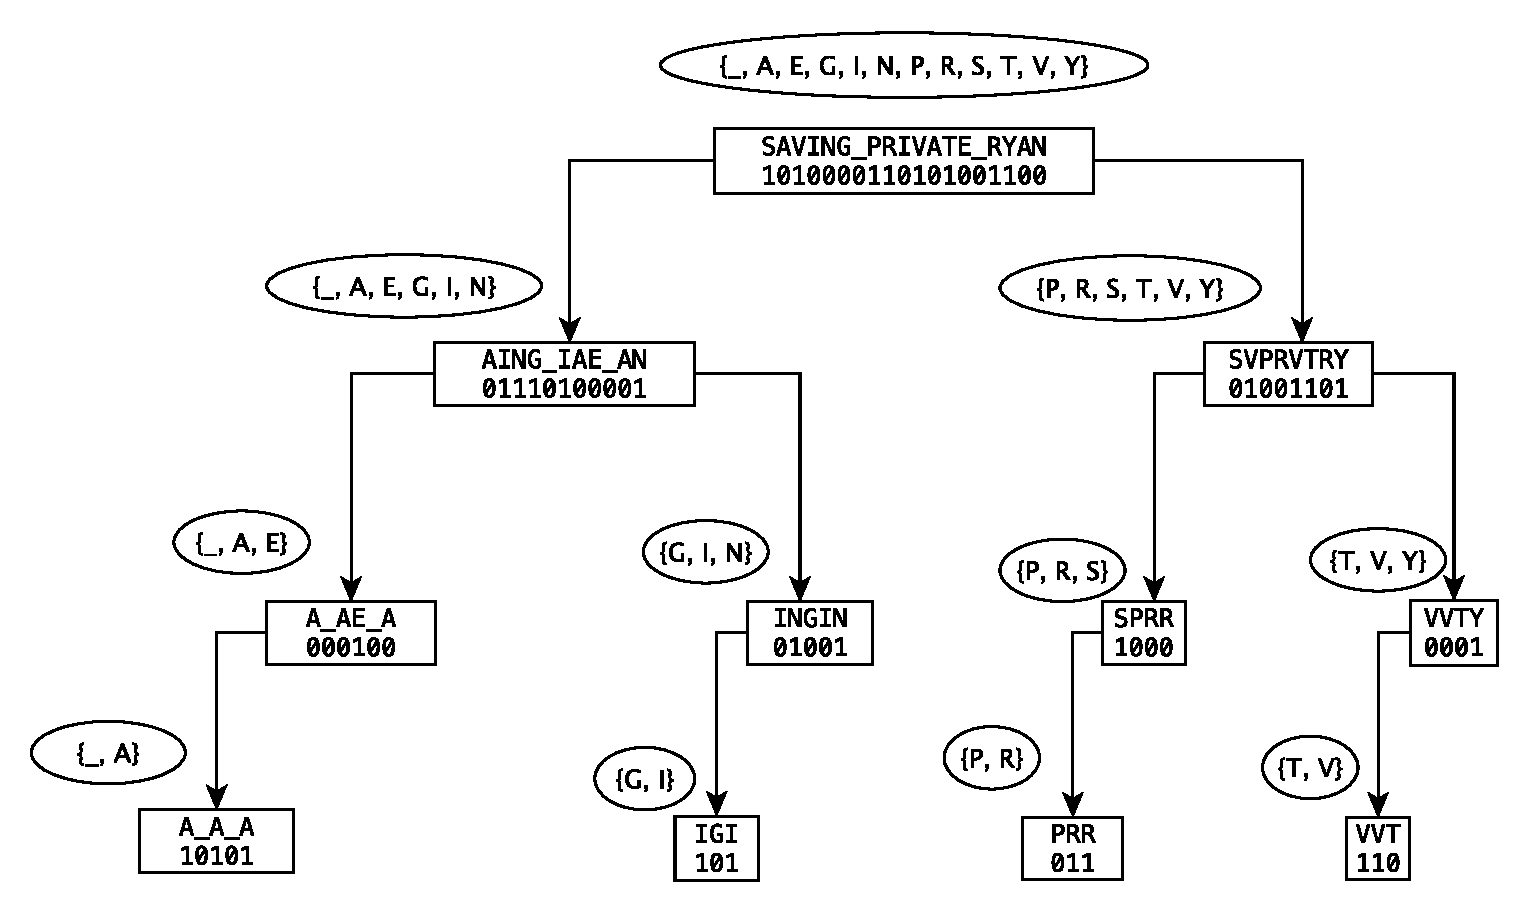
\includegraphics[width=0.9\textwidth]{img/wavelet_tree.pdf}
	\caption{Binarno stablo valića za niz \emph{Saving private Ryan}}
	\label{fig:wavelet_tree}
\end{figure}

\begin{algorithm}[H]
  \floatname{algorithm}{Pseudokod}
  \caption{Izgradnja čvora binarnog stabla valića, preuzeto iz \cite{breberic}}
  \begin{algorithmic}[1]
    \Function{izgradi}{$\Sigma, S$}
    \State Podijeli abecedu $\Sigma$ na dva jednaka dijela $\Sigma_1$ i $\Sigma_2$
    \State Kodiraj sve znakove $c \in \Sigma_1$ u nizu $S$ s 0, a ostale s 1
    \If{$|\Sigma_1| \geq S$}
      \State $S_1 \gets$ znakovi kodirani $0$ iz $S$ \State{}
      \Call{izgradi}{$\Sigma_1$, $S1$}
    \EndIf
    \If{$|\Sigma_2| \geq S$}
      \State $S_2 \gets$ znakovi kodirani $1$ iz $S$ \State{}
      \Call{izgradi}{$\Sigma_2$, $S2$}
    \EndIf
    \EndFunction
  \end{algorithmic}
  \label{alg:wnode_construct}
\end{algorithm}

\section{Upiti nad stablom valića}

Nad stablom valića definirani su sljedeći upiti:

\begin{itemize}
    \item $rank_c(i)$ - broj pojavljivanja znaka $c$ do pozicije $i$ u ulaznom nizu znakova
    \item $select_c(i)$ - pozicija $i$-tog znaka $c$ u ulaznom nizu znakova
    \item $access_c(i)$ - znak na $i$-toj poziciji u ulaznom nizu znakova
\end{itemize}

\subsection{\emph{Rank}}

\emph{Rank} upit za dani znak $c$ i poziciju $i$ ispituje koliko znakova $c$ se pojavljuje do pozicije $i$, uključeno s $i$-tom pozicijom. Algoritam je prikazan pseudokodom \ref{alg:wnode_rank}.

\begin{algorithm}[H]
  \floatname{algorithm}{Pseudokod}
  \caption{\emph{Rank} upit nad stablom valića, preuzeto iz \cite{breberic}}
  \begin{algorithmic}[1]
    \Function{rank}{$c, i$}
    \State $v \gets $ korijen stabla
    \State $r \gets i$
    \While{$v \neq null$}
      \If{$v \neq korijen$} \State $r \gets r - 1$ \EndIf
      \If{$c \in \Sigma_1$}
        \State $r \gets$ \Call{rank0}{$r$}
        \State $v \gets v_{lijevo}$
      \Else
        \State $r \gets$ \Call{rank1}{$r$}
        \State $v \gets v_{desno}$
      \EndIf
      \If{$r = 0$} \Return 0 \EndIf
    \EndWhile \State{}
    \Return $r$
    \EndFunction
  \end{algorithmic}
  \label{alg:wnode_rank}
\end{algorithm}

\subsection{\emph{Select}}

\emph{Select} upit za dani znak $c$ i broja pojavljivanja znaka tog znaka $i$ ispituje na kojoj poziciji se nalazi $i$-ti znak $c$. Algoritam je prikazan pseudokodom \ref{alg:wnode_select}.

\begin{algorithm}[H]
  \floatname{algorithm}{Pseudokod}
  \caption{\emph{Select} upit nad stablom valića, preuzeto iz \cite{breberic}}
  \begin{algorithmic}[1]
    \Function{select}{$c, i$}
    \State $v \gets $ čvor koji predstavlja znak $c$
    \State $r \gets i$
    \If{$c \in \Sigma_1$}
      \State $r \gets $ \Call{select0$_v$}{$r$}
    \Else
      \State $r \gets $ \Call{select1$_v$}{$r$}
    \EndIf
    \While{$v \neq $ korijen}
      \State $r \gets r + 1$
      \State $p \gets $ \Call{roditelj}{v}
      \If{$v$ lijevo dijete od $p$}
        \State $r \gets $ \Call{select0$_p$}{$r$}
      \Else
        \State $r \gets $ \Call{select1$_p$}{$r$}
      \EndIf
      \State $v \gets p$ 
    \EndWhile \State{}
    \Return $r$
    \EndFunction
  \end{algorithmic}
  \label{alg:wnode_select}
\end{algorithm}

\subsection{\emph{Access}}

\emph{Access} upit za danu pozicijiu $i$ vraća $i$-ti znak sekvence. Algoritam je prikazan pseudokodom \ref{alg:wnode_access}.

\begin{algorithm}[H]
  \floatname{algorithm}{Pseudokod}
  \caption{\emph{Access} upit nad stablom valića, preuzeto iz \cite{breberic}}
  \begin{algorithmic}[1]
    \Function{Access}{$i$}
    \State $v \gets $ korijen stabla
    \State $r \gets i$
    \While{$v \neq null$}
      \If{$v \neq korijen$} \State $r \gets r - 1$ \EndIf
      \If{\Call{access}{r} $= 0$}
        \State $r \gets $ \Call{rank0}{$r$}
        \If{$v_{lijevo} = null$} \Return prvi znak iz $\Sigma_v$ \EndIf
        \State $v \gets v_{lijevo}$
      \Else
        \State $r \gets $ \Call{rank1}{$r$}
        \If{$v_{desno} = null$} \Return zadnji znak iz $\Sigma_v$ \EndIf
        \State $v \gets v_{desno}$
      \EndIf
    \EndWhile\State{}
    \Return $r$
    \EndFunction
  \end{algorithmic}
  \label{alg:wnode_access}
\end{algorithm}


\chapter{Testiranje i rezultati}
U ovom poglavlju predstavljeni su rezultati memorijskih i vremenskih mjerenja te su uspoređeni s prošlogodišnjom implementacijom \cite{breberic}. Mjerenja su napravljena na umjetnim i stvarnim podacima. Prilikom provedbe mjerenja diverizfikacija je postignuta različitim veličinama abecede i ulaznih sekvenci.

Sva prikazana mjerenja su dobivena na \emph{macOS High Sierra} operativnom sustavu te procesoru \emph{Intel® Core™ i7-7660U}. Sve izvršne datoteke, one naše i od kolega prošlogodišnje implementacije, su prevedene u \emph{release} konfiguraciji, što znači da je izvršni kod optimiran.

Umjetno stvoreni podaci su preuzeti od prošlogodišnjeg projekta \cite{breberic} te su sastavljeni od različitih kombinacija veličine abecede i ulaznog niza. Tako su prisutne veličine abecede $4$, $15$ i $26$ te duljine ulaznih nizova: $100, 1.000, 10.000, 100.000$ i $1.000.000$. Stvarni podaci su \emph{FASTA} datoteke preuzete s javno dostupnih baza genoma te je njihova statistika prikazana u tablici \ref{table:fasta_file_stats}.

\begin{table}[H]
  \centering
  \caption{Statistike za FASTA datoteke}
  \begin{tabular}{P{2.5cm}P{3cm}P{3cm}}
    \toprule
    Datoteka 	& Duljina niza      & Veličina abecede \\ \hline
    HIV 		& $999$	 			& $5$ \\ \hline
    E Coli 		& $5.534.367$ 		& $4$ \\ \hline
    Flu 		& $3.990$			& $4$ \\ \hline
    Camelpox 	& $205.719$ 		& $4$ \\ \hline
    Bact1 		& $1.587.120$ 		& $4$ \\
    \bottomrule
  \end{tabular}
  \label{table:fasta_file_stats}
\end{table}

\section{Memorijska mjerenja}

Tablice \ref{table:tree_mem_synt} i \ref{table:tree_mem_fasta} prikazuju zauzeće memorije stabla u dvije inačice, kodirana i nekodirana. Kodirana inačica sadrži RRR strukture koje su kodirane kako je prethodno opisano, dok nekodirana inačica ne sadrži kodirane RRR strukture, već zapisuje rang i odmak kao standardne brojeve. Tablica \ref{table:tree_mem_synt} sadrži mjerenja za umjetno stvorene nizove, dok \ref{table:tree_mem_fasta} sadrži mjerenja za stvarne nizove.

\begin{table}[H]
\centering
\caption{Potrošnja memorije stabla valića za umjetno stvorene nizove}
  \begin{tabular}{r*{6}{P{1.5cm}}}
    \toprule
    \multirow{3}{1.5cm}[-0.5em]{\centering Duljina sekvence} &  \multicolumn{6}{c}{Veličina abecede} \\
    \cmidrule(lr){2-7} 
    			& 4 & 15 & 26 & 4 & 15 & 26 \\
    \cmidrule(lr){2-7} 
    			& \multicolumn{3}{c}{Kodiran ($kB$)} & \multicolumn{3}{c}{Nekodiran ($kB$)} \\
    \hline
    100 		& $24$ & $32$ & $40$ & $24$ & $32$ & $44$ \\ \hline
    1000		& $28$ & $44$ & $56$ & $28$ & $48$ & $64$ \\ \hline
    10000		& $60$ & $140$ & $196$ & $140$ & $200$ & $264$ \\ \hline
    100000		& $420$ & $640$ & $1.088$ & $712$ & $1.400$ & $1.600$ \\ \hline
    1000000		& $3.608$ & $5.488$ & $7.152$ & $4.848$ & $8.164$ & $10.352$ \\
    \bottomrule
  \end{tabular}
  \label{table:tree_mem_synt}
\end{table}

\begin{figure}[ht]
	\centering
	\includegraphics[width=1.0\textwidth] {graphs/graph1.png}
	\caption{Memorija stabla valića za umjetno stvorene nizove}
	\label{fig:tree_mem_synt}
\end{figure}

\begin{table}[H]
\centering
  \caption{Potrošnja memorije stabla valića za \emph{FASTA} datoteke}
  \begin{tabular}{P{2.5cm}*{2}{P{3.5cm}}}
    \toprule
    Datoteka & Kodiran ($kB$) & Nekodiran ($kB$) \\ \hline
    HIV 		& $32$ & $32$ \\ \hline
    E Coli 		& $16.240$ & $24.728$ \\ \hline
    Flu 		& $36$ & $52$ \\ \hline
    Camelpox	& $900$ & $1.008$ \\ \hline
    Bact1 		& $4.776$ & $7.312$ \\ 
    \bottomrule
  \end{tabular}
  \label{table:tree_mem_fasta}
\end{table}

Iz tablica \ref{table:tree_mem_synt} i \ref{table:tree_mem_fasta} vidljivo je da za stabla koja koriste kodiranje zauzimaju manje memorije kod većih sekvenci, od $30\%$ do $60\%$ manje memorije. Iako je zauzeće memorije manje, kodiranje uzima svoj danak prilikom izvođenja upita što je prikazano u sljedećem pod-poglavlju.

\section{Vremenska mjerenja}

Tablice \ref{table:tree_time_synt} i \ref{table:tree_time_fasta} prikazuju vrijeme potrebno za izgradnju stabla dvije inačica, kodirana i nekodirana. Tablica \ref{table:tree_time_synt} sadrži mjerenja za umjetno stvorene nizove, dok \ref{table:tree_time_fasta} sadrži mjerenja za stvarne nizove. Iz tablice \ref{table:tree_time_synt} vidljivo je kako je više vremena potrebno za izgradnju stabla sa kodiranjem za veće sekvence s većom abecedom, dok je iz tablice \ref{table:tree_time_fasta} vidljivo kako jedino za HIV potrebno više vremena za izgradnju stabla bez kodiranja, no razlika je zanemariva i vjerojatno je posljedica nepreciznosti mjerene metode.

\begin{table}[H]
\centering
\caption{Vrijeme izgradnje stabla valića za umjetno stvorene datoteke}
  \begin{tabular}{r*{6}{P{1.5cm}}}
    \toprule
    \multirow{3}{1.5cm}[-0.5em]{\centering Duljina sekvence} &  \multicolumn{6}{c}{Veličina abecede} \\
    \cmidrule(lr){2-7} 
    			& 4 & 15 & 26 & 4 & 15 & 26 \\
    \cmidrule(lr){2-7} 
    			& \multicolumn{3}{c}{Kodiran ($\mu{}s$)} & \multicolumn{3}{c}{Nekodiran ($\mu{}s$)} \\
    \hline
    100 		& $61$ & $136$ & $120$ & $61$ & $96$ & $136$ \\ \hline
    1000		& $118$ & $244$ & $280$ & $116$ & $215$ & $293$ \\ \hline
    10000		& $598$ & $1.349$ & $1.516$ & $596$ & $1.133$ & $1.478$ \\ \hline
    100000		& $5.536$ & $9.966$ & $12.819$ & $6.023$ & $14.074$ & $12.490$ \\ \hline
    1000000		& $54.351$ & $111.773$ & $133.642$ & $57.810$ & $105.501$ & $132.749$ \\
    \bottomrule
  \end{tabular}
  \label{table:tree_time_synt}
\end{table}

\begin{figure}[ht]
	\centering
	\includegraphics[width=1.0\textwidth] {graphs/graph0.png}
	\caption{Vrijeme izgradnje stabla valića za umjetno stvorene nizove}
	\label{fig:tree_time_synt}
\end{figure} 

\begin{table}[H]
\centering
  \caption{Vrijeme izgradnje stabla valića za FASTA datoteke}
  \begin{tabular}{P{2.5cm}*{2}{P{3.5cm}}}
    \toprule
    Datoteka & Kodiran ($\mu{}s$) & Nekodiran ($\mu{}s$) \\ \hline
    HIV 		& $118$           & $182$ \\ \hline
    E Coli 		& $313.131$       & $284.176$ \\ \hline
    Flu 		& $346$           & $248$ \\ \hline
    Camelpox	& $9.086$         & $8.647$ \\ \hline
    Bact1 		& $83.498$        & $77.282$ \\ 
    \bottomrule
  \end{tabular}
  \label{table:tree_time_fasta}
\end{table}

Tablice \ref{table:tree_query_time_coded_synt}, \ref{table:tree_query_time_noncoded_synt} i \ref{table:tree_query_time_fasta} prikazuju rezultate izvršavanja upita nad umjetno stvorenim i stvarnim podacima, također u dvije inačice, kodiranih i nekodiranih stabla. Isti podaci iz tablica su prikazani u obliku grafa na slikama \ref{fig:tree_rank_synt}, \ref{fig:tree_select_synt}, \ref{fig:tree_access_synt}.

\begin{table}[H]
\centering
  \caption{Prosječno vrijeme izvršavanja upita za umjetno stvorene datoteke (kodiran)}
  \begin{tabular}{r*{9}{P{1cm}}}
    \toprule
    \multirow{3}{1.3cm}[-0.5em]{\centering Duljina sekvence} &  \multicolumn{9}{c}{Veličina abecede} \\
    \cmidrule(lr){2-10} 
    			& 4 & 15 & 26 & 4 & 15 & 26 & 4 & 15 & 26 \\
    \cmidrule(lr){2-10} 
   				& \multicolumn{3}{c}{rank ($ns$)} & \multicolumn{3}{c}{select ($ns$)} & \multicolumn{3}{c}{access ($ns$)} \\
    \hline
    100 		& $229$ & $524$ & $414$    & $520$ & $1.010$ & $775$    & $509$ & $1.122$ & $805$ \\ \hline
    1000		& $248$ & $474$ & $420$    & $452$ & $860$ & $790$      & $570$ & $1.110$ & $1.025$ \\ \hline
    10000		& $369$ & $534$ & $529$    & $743$ & $1.143$ & $931$    & $855$ & $1.381$ & $1.307$ \\ \hline
    100000		& $537$ & $547$ & $665$    & $869$ & $977$ & $1.183$    & $1.176$ & $1.324$ & $1.577$ \\ \hline
    1000000		& $404$ & $898$ & $1.080$  & $679$ & $1.423$ & $1.801$  & $930$ & $1.915$ & $2.346$ \\
    \bottomrule
  \end{tabular}
  \label{table:tree_query_time_coded_synt}
\end{table}

\begin{table}[H]
\centering
  \caption{Prosječno vrijeme izvršavanja upita za umjetno stvorene datoteke (nekodiran)}
  \begin{tabular}{r*{9}{P{1cm}}}
    \toprule
    \multirow{3}{1.3cm}[-0.5em]{\centering Duljina sekvence} &  \multicolumn{9}{c}{Veličina abecede} \\
    \cmidrule(lr){2-10} 
    			& 4 & 15 & 26 & 4 & 15 & 26 & 4 & 15 & 26 \\
    \cmidrule(lr){2-10} 
   				& \multicolumn{3}{c}{rank ($ns$)} & \multicolumn{3}{c}{select ($ns$)} & \multicolumn{3}{c}{access ($ns$)} \\
    \hline
    100 		& $178$ & $274$ & $317$    & $442$ & $571$ & $693$    & $359$ & $535$ & $580$ \\ \hline
    1000		& $166$ & $243$ & $285$    & $351$ & $521$ & $605$    & $322$ & $507$ & $595$ \\ \hline
    10000		& $143$ & $249$ & $294$    & $302$ & $582$ & $663$    & $273$ & $486$ & $578$ \\ \hline
    100000		& $198$ & $337$ & $344$    & $526$ & $824$ & $856$    & $342$ & $596$ & $619$ \\ \hline
    1000000		& $217$ & $442$ & $734$    & $509$ & $926$ & $1.497$  & $365$ & $657$ & $1.037$ \\
    \bottomrule
  \end{tabular}
  \label{table:tree_query_time_noncoded_synt}
\end{table}

Iz priloženih grafova \ref{fig:tree_rank_synt}, \ref{fig:tree_select_synt}, \ref{fig:tree_access_synt}, izvršavanje upita je brže i do nekoliko puta bez kodiranja za sve veličine abeceda i sekvenci. Takav rezultat je i očekivan s obzirom da se dio vremena kod upita s kodiranjem potroši na dekodiranje.

\begin{figure}[H]
	\centering
	\includegraphics[width=1.0\textwidth] {graphs/graph2.png}
	\caption{Prosjećno vrijeme rank upita za umjetno stvorene nizove}
	\label{fig:tree_rank_synt}
\end{figure} 

\begin{figure}[H]
	\centering
	\includegraphics[width=1.0\textwidth] {graphs/graph3.png}
	\caption{Prosjećno vrijeme select upita za umjetno stvorene nizove}
	\label{fig:tree_select_synt}
\end{figure} 

\begin{figure}[H]
	\centering
	\includegraphics[width=1.0\textwidth] {graphs/graph4.png}
	\caption{Prosjećno vrijeme access upita za umjetno stvorene nizove}
	\label{fig:tree_access_synt}
\end{figure} 

\begin{table}[H]
\centering
\caption{Prosječno vrijeme izvršavanja upita za FASTA datoteke}
  \begin{tabular}{r*{6}{P{1.5cm}}}
    \toprule
    \multirow{3}{1.5cm}[-0.5em]{\centering Duljina sekvence} &  \multicolumn{6}{c}{Veličina abecede} \\
    \cmidrule(lr){2-7} & \multicolumn{3}{c}{Kodiran ($ns$)} & \multicolumn{3}{c}{Nekodiran ($ns$)} \\
    \cmidrule(lr){2-7} & rank & select & access & rank & select & access \\
    \hline
    HIV 		& $248$ & $451$ & $587$ & $251$ & $522$ & $507$ \\ \hline
    E Coli		& $473$ & $710$ & $982$ & $277$ & $532$ & $395$ \\ \hline
    Flu 		& $233$ & $412$ & $551$ & $142$ & $310$ & $279$ \\ \hline
    Camelpox	& $328$ & $605$ & $787$ & $152$ & $416$ & $277$ \\ \hline
    Bact1		& $396$ & $643$ & $893$ & $220$ & $465$ & $328$ \\
    \bottomrule
  \end{tabular}
  \label{table:tree_query_time_fasta}
\end{table}

Tablica \ref{table:tree_time_fasta} sadrži mjerenja vremena upita za stvarne nizove za implementacije s kodiranjem i bez kodiranja. Kao i na umjetno stvorenim datotekama, i na stvarnim datotekama kodiranje višestruko uspori izvođenje upita.

\section{Rezultati implementacije Brebrić, Kelemen, Volarić Horvat \cite{breberic}}

U nastavku su prikazani rezultati prošlogodišnjeg projekta \cite{breberic}.
U tablicama \ref{table:tree_mem_kel_synt} i \ref{table:tree_mem_kel_fasta} su prikazana memorijska zauzeća stabla valića. Kolege su također koristili kodiranje zapisa te su njihovi rezultati mjerenja nešto bolji, no razlog tomu leži u korištenju manje memorijske preciznosti i \emph{bug}-a u njihovom programu, te se to može uočiti na \emph{E Coli} mjerenjima u tablici \ref{table:tree_mem_kel_fasta} gdje njihov program ``podivlja'' na nizovima preko nekoliko milijuna znakova.

\begin{table}[H]
\centering
\caption{Potrošnja memorije stabla valića za umjetno stvorene datoteke}
  \begin{tabular}{r*{6}{P{1.5cm}}}
    \toprule
    \multirow{3}{1.5cm}[-0.5em]{\centering Duljina sekvence} &  \multicolumn{3}{c}{Veličina abecede} \\
    \cmidrule(lr){2-4} 
    			& 4 & 15 & 26\\
    \cmidrule(lr){2-4} 
    			& \multicolumn{3}{c}{Memorija ($kB$)} \\
    \hline
        100 & $12$ & $16$ & $20$ \\ \hline
        1000 & $16$ & $20$ & $24$ \\ \hline
        10000 & $76$ & $72$ & $80$ \\ \hline
        100000 & $396$ & $416$ & $420$ \\ \hline
        1000000 & $3.584$ & $4.848$ & $5.356$ \\
    \bottomrule
  \end{tabular}
  \label{table:tree_mem_kel_synt}
\end{table}

\begin{table}[H]
\centering
  \caption{Potrošnja memorije stabla valića za FASTA datoteke}
  \begin{tabular}{P{2.5cm}*{2}{P{3.5cm}}}
    \toprule
    Datoteka & Memorija ($kB$)\\ \hline
    HIV 		& $20$ \\ \hline
    E Coli 		& $28.136$ \\ \hline
    Flu 		& $24$ \\ \hline
    Camelpox	& $888$ \\ \hline
    Bact1 		& $4.700$ \\ 
    \bottomrule
  \end{tabular}
  \label{table:tree_mem_kel_fasta}
\end{table}


U tablicama \ref{table:tree_time_kel_synt} i \ref{table:tree_time_kel_fasta} su prikazana vremena izgradnje stabla valića. Rezultati su približno jednaki našima, no njihova izgradnja stabla je također zahvaćena već spomenutim \emph{bug}-om te problemi nastaju kod jako velikih nizova, što je vidljivo kod niza \emph{E Coli} u tablici \ref{table:tree_time_kel_fasta}.

\begin{table}[H]
\centering
\caption{Vrijeme izgradnje stabla valića za umjetno stvorene datoteke}
  \begin{tabular}{r*{6}{P{1.5cm}}}
    \toprule
    \multirow{3}{1.5cm}[-0.5em]{\centering Duljina sekvence} &  \multicolumn{3}{c}{Veličina abecede} \\
    \cmidrule(lr){2-4} 
    			& 4 & 15 & 26\\
    \cmidrule(lr){2-4} 
    			& \multicolumn{3}{c}{Vrijeme izgradnje ($\mu{}s$)} \\
    \hline
        100     & $47$      & $64$      & $87$      \\ \hline
        1000    & $95$      & $163$     & $213$     \\ \hline
        10000   & $671$     & $1.329$   & $1.779$   \\ \hline
        100000  & $5.635$   & $9.563$   & $11.834$  \\ \hline
        1000000 & $52.041$  & $106.479$ & $113.794$ \\
    \bottomrule
  \end{tabular}
  \label{table:tree_time_kel_synt}
\end{table}

\begin{table}[H]
\centering
  \caption{Vrijeme izgradnje stabla valića za FASTA datoteke}
  \begin{tabular}{P{2.5cm}*{2}{P{3.5cm}}}
    \toprule
    Datoteka & Vrijeme ($\mu{}s$) \\ \hline
    HIV 		& $98$      \\ \hline
    E Coli 		& $549.105$ \\ \hline
    Flu 		& $215$     \\ \hline
    Camelpox	& $9.801$   \\ \hline
    Bact1 		& $81.731$  \\
    \bottomrule
  \end{tabular}
  \label{table:tree_time_kel_fasta}
\end{table}

U tablicama \ref{table:tree_query_time_kel_synt} i \ref{table:tree_query_time_kel_fasta} su prikazana prosječna vremena izvršavanja upita. Rezultati su približno jednaki našima s kodiranjem, čak nešto i lošija. Kolege nisu implementirali nekodiranu inačicu stabla, stoga te rezultate nije moguće usporediti, na kako je već vidljivo i u našim rezultatima, zasigurno bi bili bolji nego u slučaju kodiranih nizova. 

\begin{table}[H]
\centering
  \caption{Prosječno vrijeme izvršavanja upita za umjetno stvorene datoteke}
  \begin{tabular}{r*{9}{P{1cm}}}
    \toprule
    \multirow{3}{1.3cm}[-0.5em]{\centering Duljina sekvence} &  \multicolumn{9}{c}{Veličina abecede} \\
    \cmidrule(lr){2-10} 
    			& 4 & 15 & 26 & 4 & 15 & 26 & 4 & 15 & 26 \\
    \cmidrule(lr){2-10} 
   				& \multicolumn{3}{c}{rank ($ns$)} & \multicolumn{3}{c}{select ($ns$)} & \multicolumn{3}{c}{access ($ns$)} \\
    \hline
    100     & $235$ & $354$ & $416$     & $297$ & $411$ & $464$     & $556$     & $808$     & $889$     \\ \hline
    1000    & $268$ & $408$ & $454$     & $318$ & $474$ & $547$     & $631$     & $982$     & $1.134$   \\ \hline
    10000   & $405$ & $610$ & $715$     & $505$ & $778$ & $893$     & $977$     & $.1543$   & $1.767$   \\ \hline
    100000  & $450$ & $634$ & $739$     & $578$ & $814$ & $964$     & $.1062$   & $1.560$   & $1.841$   \\ \hline
    1000000 & $514$ & $708$ & $1.059$   & $707$ & $974$ & $1.463$   & $.1202$   & $1.753$   & $2.536$   \\
    \bottomrule
  \end{tabular}
  \label{table:tree_query_time_kel_synt}
\end{table}

\begin{table}[H]
\centering
\caption{Prosječno vrijeme izvršavanja upita za FASTA datoteke}
  \begin{tabular}{r*{4}{P{1.5cm}}}
    \toprule
    \multirow{2}{1.5cm}[-0.5em]{\centering Duljina sekvence} 
     & \multicolumn{3}{c}{Vrijeme ($ns$)} \\
    \cmidrule(lr){2-4} & rank & select & access \\
    \hline
    HIV		 & $267$     & $325$     & $653$     \\ \hline
    E Coli	 & $1.166$   & $1.583$   & $2.806$   \\ \hline
    Flu		 & $254$     & $312$     & $614$     \\ \hline
    Camelpox & $426$     & $567$     & $1.062$   \\ \hline
    Bact1	 & $504$     & $677$     & $1.138$   \\
    \bottomrule
  \end{tabular}
  \label{table:tree_query_time_kel_fasta}
\end{table}

\chapter{Opis implementacije}
Projekt je implementiran u programskom jeziku C++, programski kod dostupan je u datoteci \emph{src}. Kod koji implementira RRR strukturu nalazi se u datoteci \emph{src/rrr}, kod za binarno stablo valića u datoteci \emph{src/wavelet}, dok je kod koji sadrži pomoćne funkcije unutar datoteke \emph{src/utilty} te kod koji sadrži dijeljene definicije unutar \emph{src/shared}. Projekt je definiran \emph{Cmake} alatom koji služi za generiranje projekata za razna interaktivna razvijateljska sučelja za C++.

\subsubsection{RRRSequence}
Ovaj razred predstavlja RRR strukturu, koja se koristi za spremanje čvorova stabla valića u kodiranom ili ne kodiranom obliku. Razred sadrži metode za izvođenje upita rank0, rank1, select0, select1, access. Postoje dvije implementacije ovog razreda, jedna je pomoću kodiranja i druga bez kodiranja opisanog u prethodnom poglavlju. Implementacija bez kodiranja se nalazi na glavnoj grani git repozitroija, dok je implementacija s kodiranjem na grani feature/packing-unpacking-sequence istog repozitorija.

\subsubsection{RRRTable}
Ovaj razred je pomoćna struktura koja se koristi kod izgradnje i izvršavanja upita nad RRR strukturama. Sadrži metode za dohvat ranka0 i ranka1 na $i$-tom indeksu unutar nekog bloka, odmaka za dani rank i blok te metodu za dohvat broja bitova odmaka za dani rank.

\subsubsection{WaveletTree}
Ovaj razred predstavlja binarno stablo valića te sadrži metode za vršenje rank, select i access upita.

\subsubsection{WaveletNode}
Ovaj razred predstavlja čvor binarnog stabla valića  sadržava referencu na RRR strukturu stvorenu prilikom izgradnje stabla. Također sadrži metode za vršenje rank, select i access upita nad.

\subsubsection{bioinf\_utility}
Kod koji se koristi kod izvođenja glavnog programa za čitanje datoteka i dohvat memorije za pojedine operacijske sustave.

\subsubsection{common}
Header koji sadrži sve podatkovne tipove definirane za korištenje unutar implementacije strukture.

\subsubsection{main}
Glavna ulazna točka programa, sadrži metode za mjerenje memorije i vremena.

\chapter{Zaključak}
Pohrana i obrada ulaznih sekvenci velike duljine predstavlja pravi izazov jer u isto vrijeme želimo smanjiti potrošnju memorije i smanjiti utjecaj na performanse obrade istih. Taj problem je posebno izražen prilikom analize genetskih sekvenci, stoga je od iznimne važnosti u području bioinformatike. U ovom radu, kao struktura koja bi riješila gore navedeni problem, prikazana je implementacija statičke strukture binarnog stabla valića kao RRR strukture.

U radu je opisana teorijska podloga RRR strukture te binarnog stabla valića. Također opisana su i dva moguća pristupa prilikom izgradnje RRR strukture: kodirani i nekodirani. Kodirani pristup smanjuje memorijsko zauzeće uz mali utjecaj na performanse prilikom obavljanja upita.

Na kraju rada dani su i rezultati mjerenja i analize strukture na stvarnim i umjetnim podacima. Prava moć, to jest skalabilnost, RRR strukture vidljiva je prilikom mjerenja prosječnog vremena izvršavanja upita, gdje su se za jako velik porast duljine ulazne sekvence, i preko nekoliko milijuna znakova, vremena upita tek nešto blago linearno povećala. Memorijski rast je ipak bio nešto veći, no to je zbog same strukture stabla valića. Kao što je već spomenuto, stablo valića je statička struktura te kao takva nema mogućnost dinamičke izmjene podataka, već bi se svaki put trebalo izgraditi novo stablo, no u području bioinformatike to nam i nije neki problem jer u većini slučajeva želimo samo vršiti upite nad trenutnim podacima.

\bibliography{literatura}
\bibliographystyle{fer}

\end{document}
